\section{Research Gap: What Goes Wrong with Independent Prefetching and Partitioning}
\label{sec:problem}

\subsection{Experimental setup}
\label{sec:setup}

\begin{table}[!htbp]
\centering
\caption{Simulated system.}
\label{tab:system}
\footnotesize
\resizebox{\columnwidth}{!}{\begin{tabular}{ll}
\toprule
Simulator & ChampSim (Pythia release)~\cite{gober2022champsim,bera2021pythia} \\
Core & out-of-order, perceptron branch predictor \\
L1D / L2 & private; prefetcher at L1D+L2 (IPCP) or L2 (Pythia) \\
LLC & shared, 16 ways, 512\,KB/core (4-core: 2\,MB, 8-core: 4\,MB) \\
Partitioning & UCP~\cite{qureshi2006ucp}, 64 sampled sets, repartition every 5\,M cycles \\
DRAM & 2 channels DDR4 \\
\quad 4-core & 2400\,MT/s (9.6\,GB/s/core) and 600\,MT/s (2.4\,GB/s/core) \\
\quad 8-core & 2400\,MT/s (4.8\,GB/s/core) and 1200\,MT/s (2.4\,GB/s/core) \\
Prefetchers & IPCP (ISCA'20)~\cite{pakalapati2020ipcp}, Pythia (MICRO'21)~\cite{bera2021pythia} \\
Workloads & SPEC CPU2006/2017 traces of DPC-3~\cite{dpc3} \\
Length & 4-core: 25\,M warm-up + 100\,M; 8-core: 25\,M + 150\,M per core \\
Characterisation & 4-core, \cref{tab:char4,fig:grid}: 50\,M + 200\,M; IPCP runs 1 DRAM channel \\
\bottomrule
\end{tabular}}
\end{table}

\Cref{tab:system} lists the simulated system.  We call 2400\,MT/s \emph{ample} bandwidth.  DDR4-2400 is the
default DRAM configuration of the ChampSim release we use~\cite{gober2022champsim} and the main-memory setting of the
Pythia evaluation~\cite{bera2021pythia} (dual channel for 4 cores, as here).
The \emph{low}-bandwidth settings (600\,MT/s on 4 cores, 1200\,MT/s on 8 cores) give every core 2.4\,GB/s, a quarter
and a half of the per-core share at 2400\,MT/s.  Every single-core trace is classified by its IPC gain from more LLC
ways (high/low cache sensitivity, HC/LC) and from a more aggressive prefetcher (high/low prefetch sensitivity, HP/LP),
split at the median; borderline traces are excluded.  From the four classes HCHP, HCLP, LCHP and LCLP we build 50
four-core mixes covering every class composition (homogeneous, 2+2, 3+1, 2+1+1 and all-four) and 20 eight-core mixes
(homogeneous, 4+4, 6+2, 4+2+2, 2+2+2+2).

We report \emph{throughput} as the normalised weighted speedup: the mean over the cores of a mix of the core's IPC
divided by its IPC in a reference run of the same mix, averaged over mixes with the geometric mean.  The
\emph{harmonic speedup} (HS) is the harmonic mean of the same ratios and rewards fairness.  A core is a
\emph{casualty} when it runs more than 2\% slower than in the same mix with no prefetching and no partitioning (plain
LRU LLC), i.e.\ when turning the two mechanisms on hurts it.

\subsection{Finding 1: on 4 cores, only per-core choices beat independent operation}
\label{sec:headroom}

\begin{table}[!htbp]
\centering
\caption{4-core characterisation runs (IPCP: one DRAM channel, Pythia: two; 50\,M + 200\,M instructions per core):
speedup over UCP without prefetching, and change of DRAM reads and LLC miss latency with prefetching.}
\label{tab:char4}
\footnotesize
\resizebox{\columnwidth}{!}{\begin{tabular}{lrcccccc}
\toprule
 & & \multicolumn{2}{c}{Weighted speedup} & \multicolumn{2}{c}{Worst core} & DRAM reads & LLC miss lat. \\
\cmidrule(lr){3-4}\cmidrule(lr){5-6}
Prefetcher & Mixes & PF only & PF+UCP & PF only & PF+UCP & PF+UCP & PF+UCP \\
\midrule
Pythia & 50 & 1.393 & 1.401 & 1.003 & 1.025 & +34\% & +42\% \\
IPCP & 20 & 1.367 & 1.376 & 0.916 & 0.939 & +57\% & +60\% \\
\bottomrule
\end{tabular}
}
\end{table}

\Cref{tab:char4} shows that on 4 cores both prefetchers speed the mixes up by 37--40\% and UCP adds less than 1\% on
top.  Prefetching raises DRAM reads by 34--57\% and the average LLC miss latency by 42--60\%, and with IPCP the worst
core of a mix already loses 6--8\%.  The question is whether setting the two mechanisms \emph{together} could do
better than running them independently.  We answer it with three searches of increasing power, each measured against
the independent run (native prefetcher on every core, UCP partitioning):
\begin{enumerate}
  \item \textbf{Uniform knobs} (\cref{fig:grid}): every combination of one prefetch degree cap for all cores (native,
        4, 2, 1, off) and one partitioning policy (UCP, none, equal ways), 15 configurations on 20 (IPCP) and 26
        (Pythia) mixes.
  \item \textbf{Per-core static oracle} (\cref{fig:oracle,fig:scatter}): a greedy search over a separate degree
        cap per core (0, 1, 2, 4, native) and a fixed way allocation per core (moves of 2--4 ways), on 14 mixes per
        prefetcher.  The search is run three times, tuning only the prefetch knob (UCP partitions), only the
        partition (native prefetchers) or both; the best configurations are then re-validated at full length.
  \item \textbf{The same oracle on 8 cores} at 2.4\,GB/s per core (\cref{sec:scale}).
\end{enumerate}

\begin{figure*}[!tp]
\centering
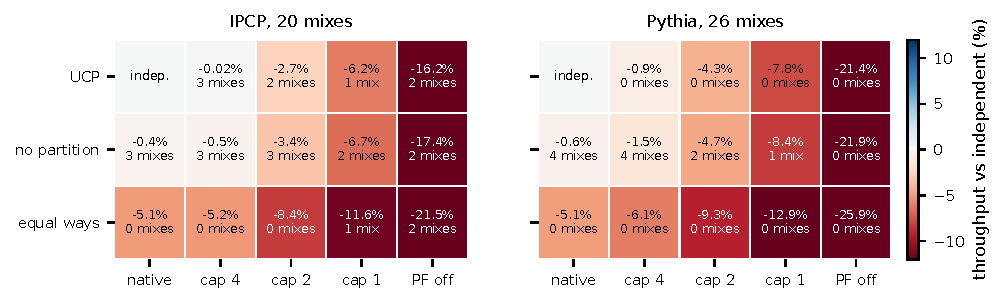
\includegraphics[width=0.92\textwidth]{grid_headroom.pdf}
\caption{Uniform knobs, 4-core: throughput of every combination of a degree cap applied to all cores and a
partitioning policy, relative to independent operation (UCP + native prefetcher, ``indep.''), geometric mean over
the mixes, and the number of mixes in which the configuration gains at least 2\%.  No uniform configuration beats
independent operation on average.}
\label{fig:grid}
\end{figure*}

\paragraph{Uniform knobs never beat independent operation}
In \cref{fig:grid} every cell is at or below independent operation: the best uniform configuration (degree cap 4
with UCP for IPCP, native Pythia without partitioning) is within 0.6\% of it, caps 2 and 1 lose 2.7--12.9\%,
switching prefetching off loses 16--26\%, and equal way allocation loses 5.1\% even with native prefetchers.  A
uniform cap also hurts fairness: the mean worst core of a mix drops to 0.98, 0.89 and 0.81 of its independent IPC
at caps 4, 2 and 1 (IPCP; Pythia 0.97, 0.90, 0.82).  A uniform configuration helps only in a few mixes (at most 4 of 20 or 26 per cell).  Even an oracle that picks the best uniform configuration per mix gains only
3.3\% (IPCP) and 0.4\% (Pythia); the IPCP mean is carried by a single mix (mix 9, +39\% with prefetching off)
in this one-channel setup.

\begin{table}[!htbp]
\centering
\caption{Headroom over independent PF+UCP (throughput).  Uniform knobs: best of the 15 configurations of
\cref{fig:grid} chosen per mix.  Per-core oracle: best validated per-core degree caps $\times$ way allocation.}
\label{tab:oracle}
\footnotesize
\resizebox{\columnwidth}{!}{\begin{tabular}{lllrccc}
\toprule
Search & Setup & PF & Mixes & Mean & Max & $\geq$+3\% \\
\midrule
Uniform knobs & 4-core, 1 ch. & IPCP & 20 & +3.3\% & +39.2\% & 4 \\
Uniform knobs & 4-core, 2 ch. & Pythia & 26 & +0.4\% & +6.0\% & 2 \\
\midrule
Per-core oracle & 4-core, 9.6\,GB/s & IPCP & 14 & +4.6\% & +17.2\% & 7 \\
Per-core oracle & 4-core, 9.6\,GB/s & Pythia & 14 & +1.1\% & +5.4\% & 2 \\
Per-core oracle & 8-core, 2.4\,GB/s & IPCP & 8 & +14.9\% & +38.2\% & 6 \\
\bottomrule
\end{tabular}
}
\end{table}

\begin{figure*}[!tp]
\centering
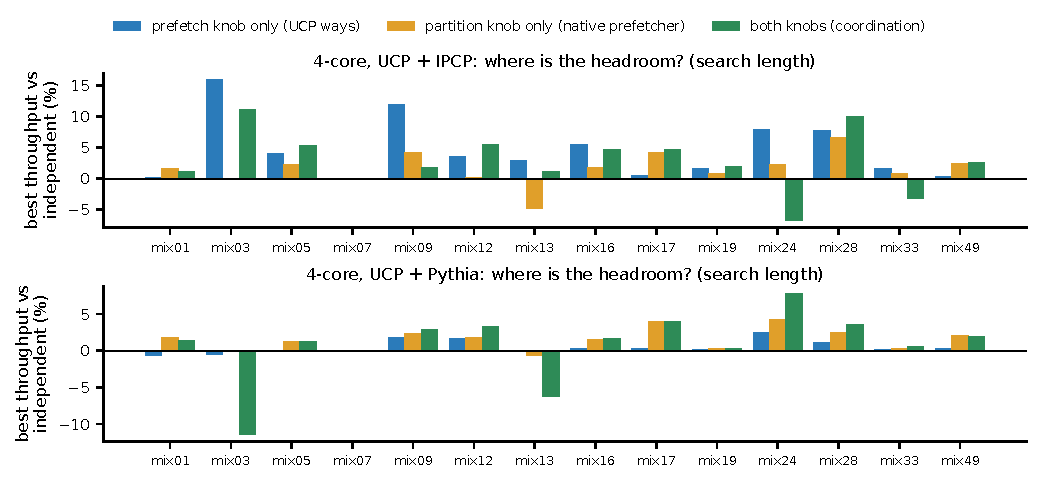
\includegraphics[width=0.9\textwidth]{oracle_knobs.pdf}
\caption{Per-core static oracle, 4-core, 9.6\,GB/s/core: where is the headroom?  Best throughput over independent
operation when only the prefetch knob (UCP keeps partitioning), only the partition knob (native prefetchers) or both
are searched, at the search length.  A missing bar: no configuration of that search was evaluated.}
\label{fig:oracle}
\end{figure*}

\begin{figure*}[!tp]
\centering
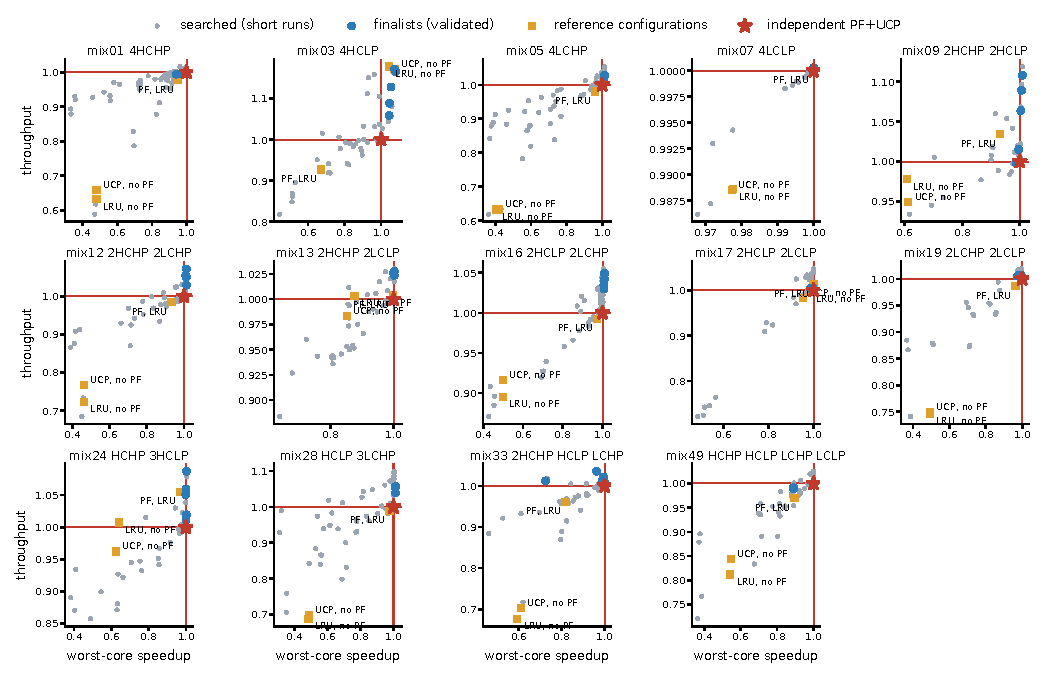
\includegraphics[width=0.9\textwidth]{oracle_scatter_ipcp.pdf}
\caption{Per-core static oracle, 4-core, 9.6\,GB/s/core, UCP+IPCP: every fixed configuration evaluated, as
throughput against the speedup of the worst core, both relative to independent operation (star).  Grey: searched
configurations (short runs); blue: finalists re-validated at full length; orange: prefetching alone on LRU, UCP alone
and neither.  Up and to the right of the star is better.}
\label{fig:scatter}
\end{figure*}
\paragraph{Per-core decisions find headroom with IPCP, and need both knobs}
Choosing a degree cap and a way allocation per core (\cref{tab:oracle}) finds \OrcIpMean\% (IPCP) and
\OrcPyMean\% (Pythia) on average after validation, at most \OrcMax\%, and at least 3\% in \OrcIpThree{} of \OrcIpN{}
IPCP mixes but only \OrcPyThree{} of \OrcPyN{} Pythia mixes.  \Cref{fig:scatter} (IPCP; Pythia in \cref{fig:scatterpy}, appendix) shows every configuration
the search evaluated.  With Pythia, the best validated configuration is within 1.5\% of independent operation in
12 of 14 mixes.  \Cref{fig:oracle} decomposes the search.  The two prefetchers need different knobs: for IPCP the prefetch knob alone is worth \KnIpPf\%
at the search length and the partition alone \KnIpPart\%, for Pythia, which already adapts to bandwidth, the partition is
worth more (\KnPyPart\% against \KnPyPf\%).  In \KnIpBoth{} (IPCP) and \KnPyBoth{} (Pythia) of the \KnIpN{} mixes the best configuration sets
\emph{both} knobs.  The joint search sometimes ends in a worse configuration than either single-knob search (\KnFragile), and part of the search-length gain disappears at full length (IPCP: \KnIpBest\% on \KnIpN{} mixes at
search length, \OrcIpMean\% on the \OrcIpN{} validated mixes).  On 4 cores with ample bandwidth the per-core oracle thus finds headroom mainly in the prefetch knob with IPCP and
in the partition with Pythia.

\subsection{Finding 2: with less bandwidth per core, prefetching creates casualties}
\label{sec:scale}

\begin{table}[!htbp]
\centering
\caption{8-core factorial study (20 mixes): throughput vs no prefetching and no partitioning, max slowdown,
fairness, and casualty cores (of 160).}
\label{tab:scaleup}
\footnotesize
\resizebox{\columnwidth}{!}{\begin{tabular}{llrcccc}
\toprule
DRAM & Configuration & PF & Thr. vs no-PF & Max slowdown & Fairness & Casualties \\
\midrule
2400 MT/s & No PF, no partitioning & -- & 1.000 & 2.02 & 0.57 & 0 \\
2400 MT/s & UCP only & -- & 1.004 & 2.03 & 0.57 & 23 \\
2400 MT/s & PF only (LRU) & IPCP & 1.220 & 2.05 & 0.42 & 45 \\
2400 MT/s & PF only (LRU) & Pythia & 1.309 & 1.89 & 0.43 & 33 \\
2400 MT/s & PF + UCP & IPCP & 1.221 & 2.11 & 0.41 & 47 \\
2400 MT/s & PF + UCP & Pythia & 1.307 & 1.79 & 0.44 & 32 \\
\midrule
1200 MT/s & No PF, no partitioning & -- & 1.000 & 2.18 & 0.55 & 0 \\
1200 MT/s & UCP only & -- & 1.003 & 2.20 & 0.55 & 25 \\
1200 MT/s & PF only (LRU) & IPCP & 1.134 & 2.48 & 0.40 & 61 \\
1200 MT/s & PF only (LRU) & Pythia & 1.234 & 2.27 & 0.41 & 42 \\
1200 MT/s & PF + UCP & IPCP & 1.129 & 2.53 & 0.39 & 57 \\
1200 MT/s & PF + UCP & Pythia & 1.231 & 2.14 & 0.43 & 41 \\
\bottomrule
\end{tabular}
}
\end{table}

\begin{figure*}[!tp]
\centering
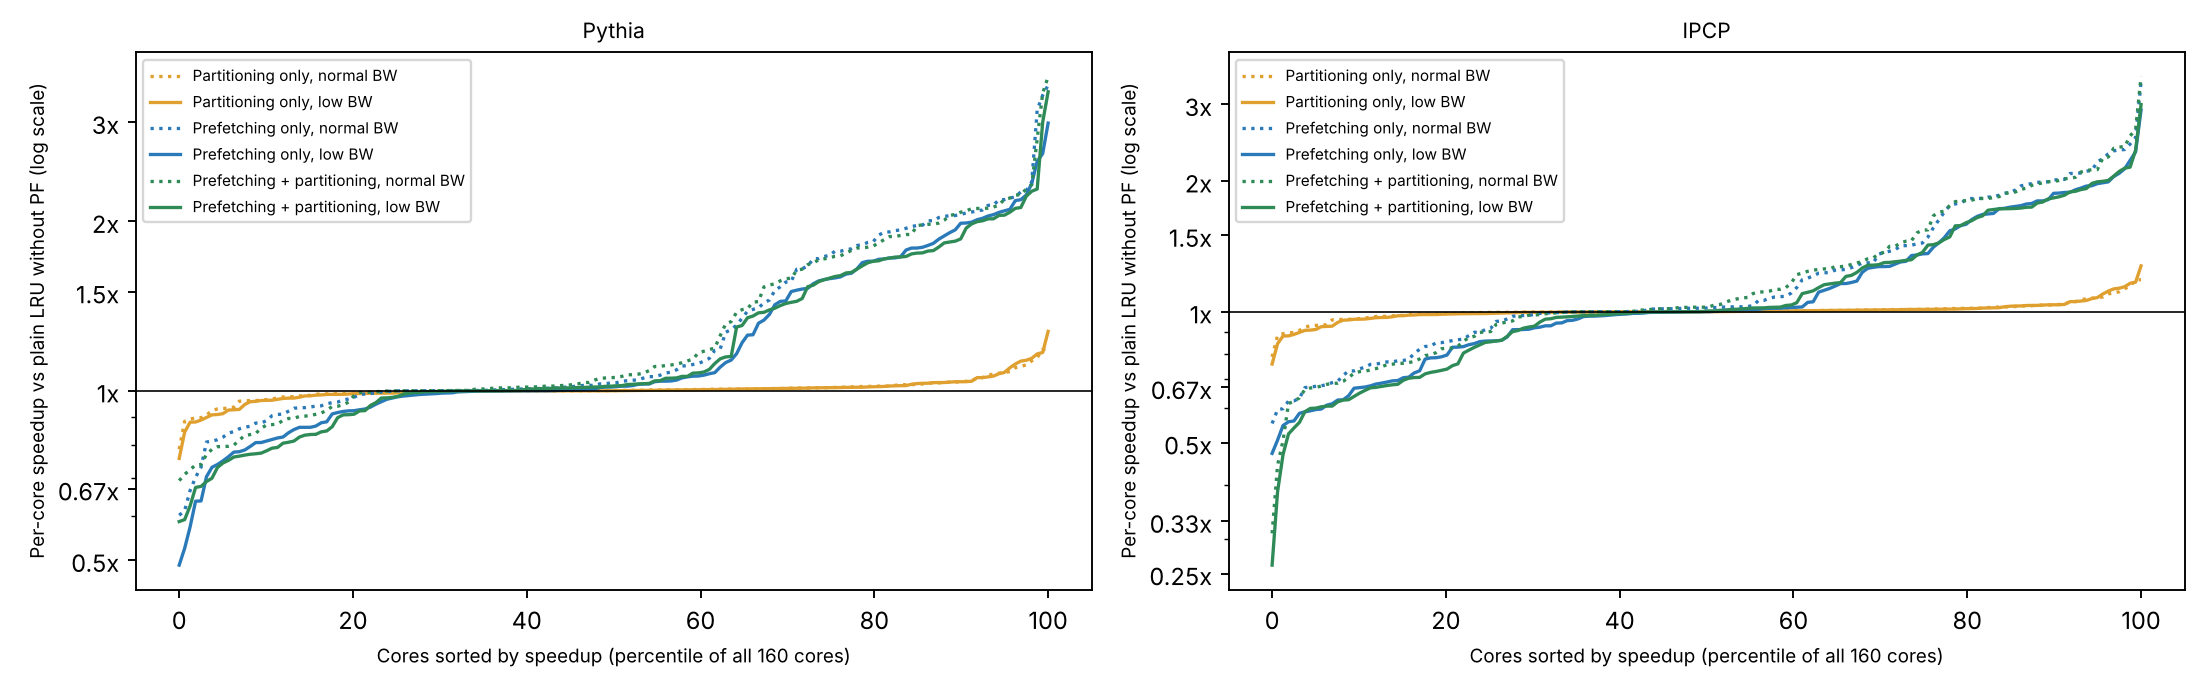
\includegraphics[width=0.8\textwidth]{percore_8core.png}
\caption{8-core: per-core speedup over plain LRU without prefetching for all 160 cores, sorted, for each mechanism
alone and both together, at 4.8 (dotted) and 2.4\,GB/s per core (solid).  The averages of
\cref{tab:scaleup} hide a left tail of cores that prefetching slows down, and the tail grows when the bandwidth per
core halves.}
\label{fig:casualties}
\end{figure*}

On 8 cores (\cref{tab:scaleup}, \cref{fig:casualties}), halving the per-core bandwidth from 4.8 to 2.4\,GB/s lowers
the throughput gain of IPCP+UCP from 22\% to 13\% and raises the casualties from 47 to 57 of 160 cores (Pythia: 32 to
41); with IPCP the worst core of a mix is slowed down 2.5$\times$ on average.  The per-core static oracle at 2.4\,GB/s per core
finds a mean headroom of 14.9\% and a maximum of 38.2\% for IPCP, at least 3\% in 6 of 8 mixes (\cref{tab:oracle};
every configuration in \cref{fig:scatter8}, appendix).  It comes almost entirely from the prefetch knob: at the
search length, tuning only the degrees reaches 19.8\% on average, tuning only the partition 4.4\%, and the joint
search, which evaluated only 16 configurations (against 144 and 88), $-2.4\%$.  In four of eight mixes the best
fixed configuration turns IPCP off on every core, which costs the worst core up to 54\%; the fairest configuration
that does not lose throughput throttles a single core in six of eight mixes and still gains 0.1--22\%.

\subsection{Finding 3: UCP barely reacts, and rewards the wrong prefetchers}

\begin{figure*}[!tp]
\centering
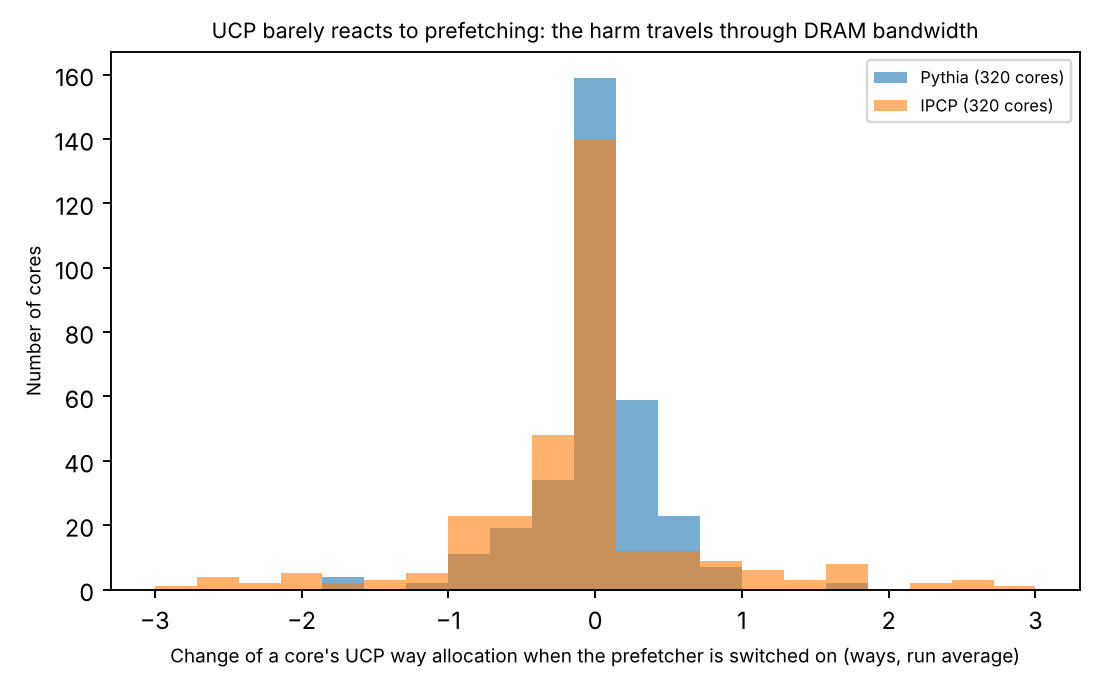
\includegraphics[height=1.75in]{realloc_8core.png}\hfill
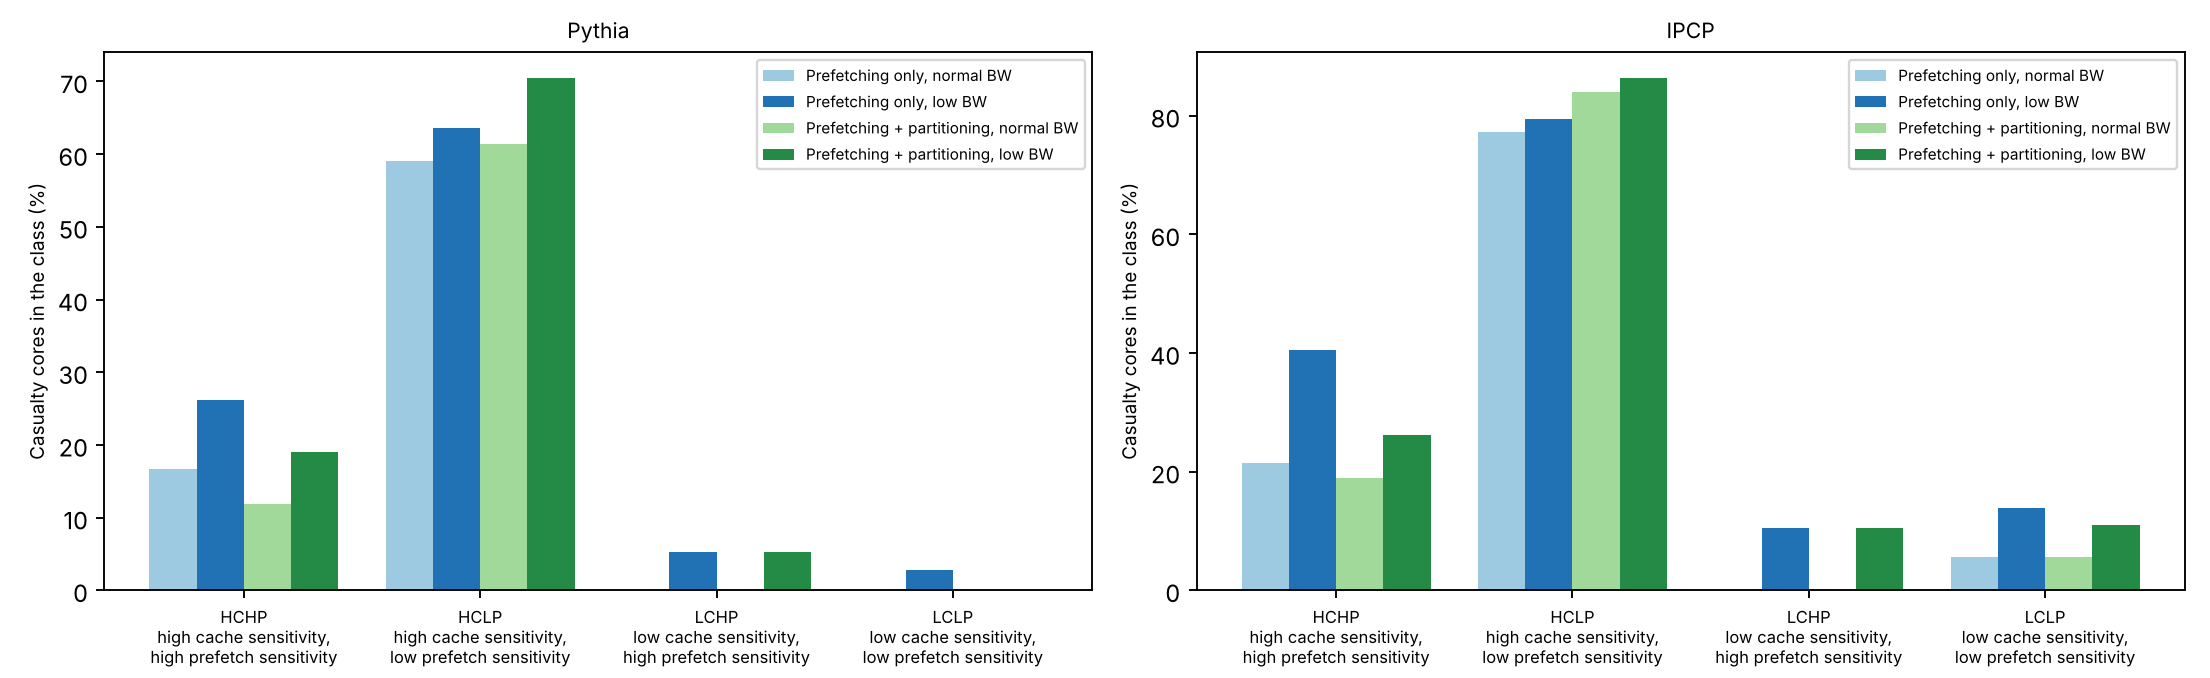
\includegraphics[height=1.75in]{byclass_8core.png}
\caption{8-core: change of each core's UCP way allocation when its prefetcher is switched on (left) and casualties by
workload class (right).
UCP changes the allocation of few cores; the casualties are mostly cache-sensitive (HC) cores.}
\label{fig:interaction}
\end{figure*}

Enabling the prefetcher changes the average UCP allocation of a core by at least one way for only 54 of 320
(IPCP) and 8 of 320 (Pythia) cores (\cref{fig:interaction}, left).
Where UCP does react, it reacts the wrong way: with IPCP, the 31 cores that gain at least one way have a median
prefetch accuracy of 0.08 (against 0.29 over all cores), and all 23 cores that lose at least one way are
cache-sensitive (15 HCLP, 8 HCHP).  The casualties concentrate in exactly these classes (\cref{fig:interaction},
right).  In 39--49\% (IPCP) and 33--41\% (Pythia) of the cores, enabling both mechanisms is worse than the better of
the two alone.

\subsection{Finding 4: why prior-style throttling loses throughput}

\begin{figure*}[!tp]
\centering
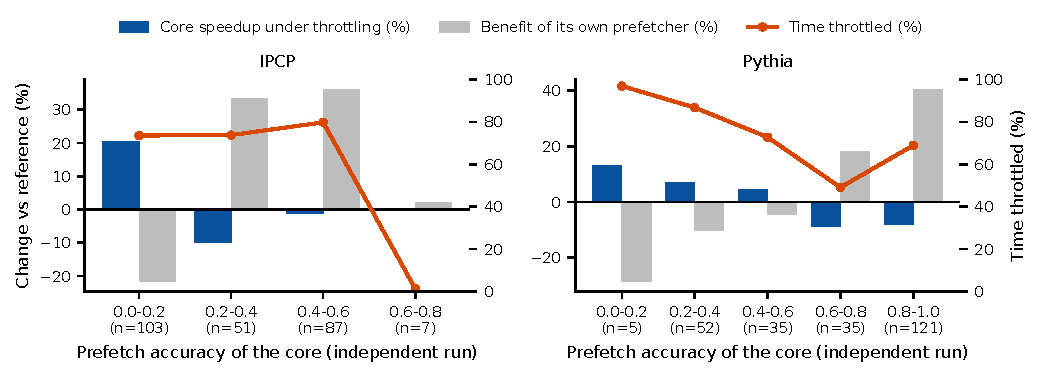
\includegraphics[width=0.9\textwidth]{root_cause_accuracy.pdf}
\caption{Fairness-driven throttling (FDT: keep a throttle step when the fairness score improves), 4-core 2.4\,GB/s/core
and 8-core cores grouped by their prefetch accuracy.  Blue: the core's speedup under FDT over independent operation; grey: the
core's speedup in the independent run over neither prefetching nor partitioning; line: share of time FDT kept it
throttled.  On average the inaccurate cores (accuracy below about 0.2 for IPCP, 0.6 for Pythia) gain and the accurate
ones lose.}
\label{fig:rootcause}
\end{figure*}

We implemented a feedback throttling controller in the spirit of HPAC~\cite{ebrahimi2009hpac}, which we call
\emph{fairness-driven throttling} (FDT): every epoch it
detects DRAM pressure, tentatively lowers the prefetch level of the core with the most useless (or the most) prefetch
traffic, and keeps the step if the weighted harmonic mean of all cores' IPC improves.  It gains up to 41\% on some mixes
(+28\%, +36\% and +41\% on three 8-core IPCP mixes), but loses up to 11.5\% on a 4-core mix and 15.7\% on an 8-core
mix, with 5 of 22 4-core mixes below $-2\%$ for IPCP and 7 for Pythia.  \Cref{fig:rootcause} groups the cores by
prefetch accuracy: on average the inaccurate cores (accuracy below 0.2 for IPCP, 0.6 for Pythia) gain and the
accurate ones lose.  The cores that the independent run speeds up by at least 1.3$\times$ over neither mechanism (71 with IPCP, 88
with Pythia) are
kept throttled 93\% and 88\% of the time and end up 11\% and 16\% slower.  FDT keeps a step only when the fairness
score of the trial rises, so these steps passed its test although they slowed the throttled cores down.  Coordinating the partition as well (FDT+PSR, FDT+Reclaim) did not remove these losses: all three designs have 5
4-core IPCP mixes below $-2\%$ (\cref{tab:final4}).  Changing the acceptance rule did: TSC-T, which differs from FDT
mainly in its acceptance rule, has 2 such mixes.

\subsection{Problem statement}
\label{sec:statement}

Running the two mechanisms independently has three problems:
\begin{enumerate}
  \item \textbf{Prefetching slows down more cores when bandwidth per core is low.}  On 8 cores, halving the bandwidth
        per core from 4.8 to 2.4\,GB/s raises the casualties (cores more than 2\% slower than with neither prefetching
        nor partitioning) from 47 to 57 of 160 with IPCP and from 32 to 41 with Pythia (\cref{tab:scaleup}).
  \item \textbf{UCP gives ways to inaccurate prefetchers.}  UCP's monitors count every hit, including hits on
        prefetched lines~\cite{qureshi2006ucp}.  With IPCP, the cores that gain ways when prefetching is enabled have
        a median prefetch accuracy of 0.08 (0.29 over all cores), and all cores that lose ways are cache-sensitive
        (Finding~3).
  \item \textbf{Fixing one side is not enough.}  None of the 14 uniform settings of the two knobs beats independent
        operation, and degree caps of 2 or 1 lose 2.7--12.9\% (\cref{fig:grid}).  Throttling on fairness alone (FDT)
        keeps the cores that prefetching speeds up by at least 1.3$\times$ throttled about 90\% of the time; they end
        up 11--16\% slower (Finding~4, \cref{fig:rootcause}).
\end{enumerate}

\paragraph{Why two-way}
The per-core oracle (\cref{fig:oracle}, \cref{sec:headroom}) gains \KnIpPf\% (IPCP) and \KnPyPf\% (Pythia) when it
searches only the prefetch knob and \KnIpPart\% and \KnPyPart\% when it searches only the partition.  In \KnIpBoth{}
(IPCP) and \KnPyBoth{} (Pythia) of \KnIpN{} mixes the best setting it finds changes both knobs.

\paragraph{Problem}
\emph{Coordinate prefetch throttling and LLC partitioning in both directions under limited DRAM bandwidth, so that
throughput and fairness increase by removing only the prefetching that does not help its own core and by not giving
LLC ways to useless prefetches, without lowering the overall throughput.}  The controller should work with any prefetcher and any way partitioner without changing them.
